\subsection{Линейный фильтр первого порядка}

Будем рассматривать линейный фильтр первого порядка, который описывается следующим уравнением:
\begin{equation}
    W_1(p) = \frac{1}{Tp + 1}
\end{equation}
где $T$ -- постоянная времени.

\def\num{1}
\def\a{4}
\def\from{1}
\def\to{4}
\def\b{1}
\def\c{0}
\def\d{0}
\def\L{10}
\def\T{0.5}

\subsubsection{Рассматриваемая функция}
Рассмотрим функцию $g(t)$ при параметрах $a=\a$, $t_1 = \from$, $t_2 = \to$ ~(см. рисунок~\ref{fig:wave_func_\num}) 
и ее \textit{зашумленную} версию $u(t)$ с параметрами $b = \b$, $c = \c$, $d = \d$ ~(см. рисунок~\ref{fig:noised_wave_func_\num}).
на промежутке $[0,\L]$. 

\subsubsection{Графики рассматриваемой и зашумленной функции}
\begin{figure}[ht!]
    \centering
    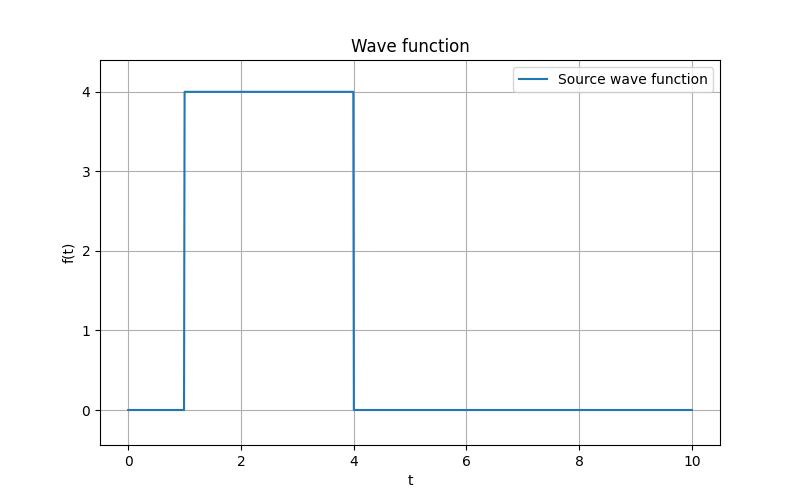
\includegraphics[width=\textwidth]{../results/second/\num/wave_func.png}
    \caption{Функция $g(t)$ с параметрами $a = \a$, $t_1 = \from$, $t_2 = \to$}
    \label{fig:wave_func_\num}
\end{figure}

\begin{figure}[ht!]
    \centering
    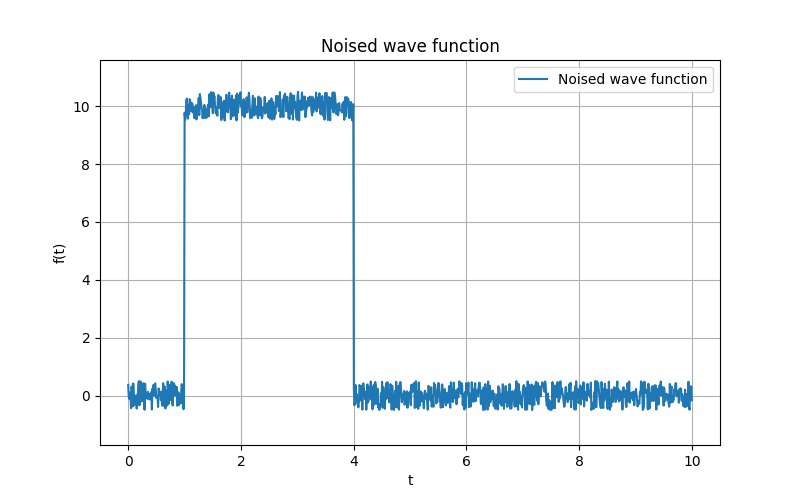
\includegraphics[width=\textwidth]{../results/second/\num/noised_wave_func.png}
    \caption{Функция $u(t)$ с параметрами $b = \b$, $c = \c$, $d = \d$}
    \label{fig:noised_wave_func_\num}
\end{figure}

\FloatBarrier
\subsubsection{Применение фильтра}

Рассмотрим фильтрованную функцию $u'(t)$, которая получается применением линейного фильтра первого порядка с $T = \T$ (см. рисунок \ref{fig:noised_wave_func_filtered_\num}).

\begin{figure}[ht!]
    \centering
    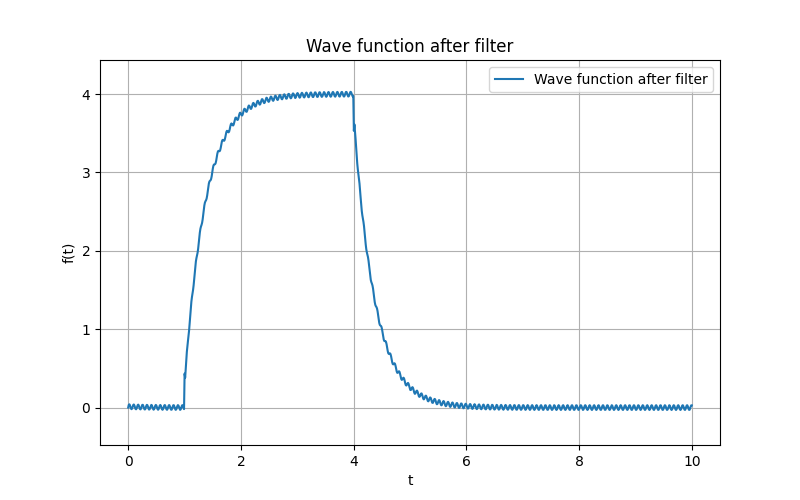
\includegraphics[width=\textwidth]{../results/second/\num/noised_wave_func_filtered.png}
    \caption{Функция $u'(t)$ после применения фильтра}
    \label{fig:noised_wave_func_filtered_\num}
\end{figure}

Видим, что функция после фильтрации стала более гладкой, фронт и спад стали менее выраженными. 
Это связано с тем, что фильтр убирает высокочастотные компоненты функции. Убедиться в этом можно 
рассмотрев АЧХ данного фильтра (см. рисунок \ref{fig:filter_frequency_response_\num}).

\FloatBarrier
\subsubsection{Аплитудно-частотная характеристика фильтра}
\begin{figure}[ht!]
    \centering
    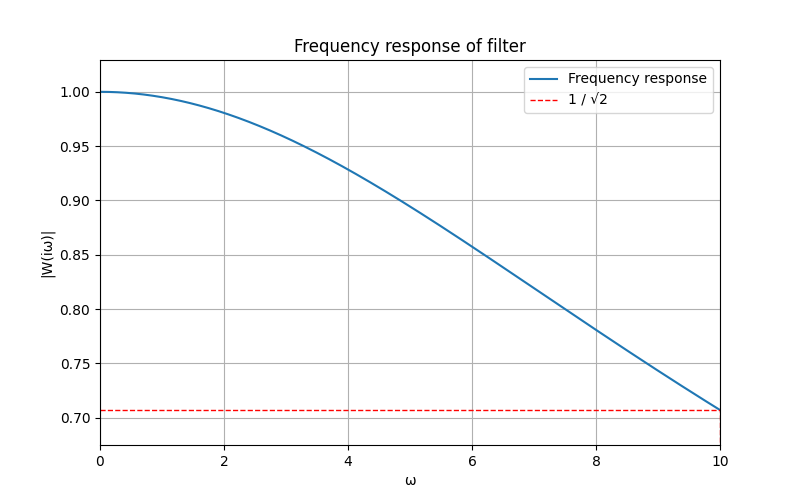
\includegraphics[width=\textwidth]{../results/second/\num/filter_frequency_response.png}
    \caption{АЧХ фильтра первого порядка при $T = \T$}
    \label{fig:filter_frequency_response_\num}
\end{figure}

На графике также отмечено значение $\omega_c$ -- \textit{частоты среза} $|W(i\omega_c)| = \frac{1}{\sqrt{2}}$, по нему можно судить о том, какие частоты будут \textit{усиливаться}, а какие \textit{подавляться}. 
Для фильтра первого порядка это значение равно $\omega_c = \frac{1}{T}$. Таким образом, делаем вывод, что все частоты, 
большие $\frac{1}{\T} = \fpeval{1/ \T}$ будут подавляться, что соответствует значению на графике. 

\FloatBarrier
\subsubsection{Результаы фильтрации}
Сравнительный график исходной функции и функции после фильтрации представлен на рисунке \ref{fig:wave_func_cmp_\num}.

\begin{figure}[ht!]
    \centering
    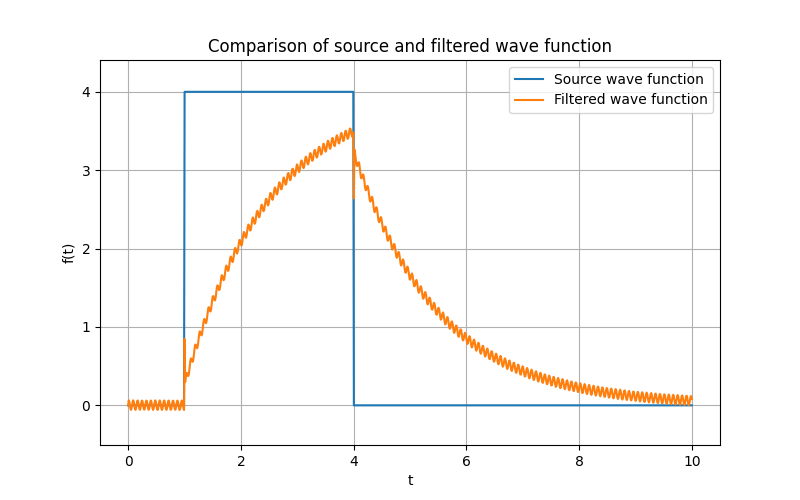
\includegraphics[width=\textwidth]{../results/second/\num/wave_func_cmp.png}
    \caption{Сравнение функции $g(t)$ и $u'(t)$}
    \label{fig:wave_func_cmp_\num}
\end{figure}

Образ исходной функции и функции после фильтрации приведены на рисунках \ref{fig:wave_func_image_\num}~и~\ref{fig:noised_wave_func_filtered_image_\num}.
Графики модулей соответствующих функций приведены на рисунках~\ref{fig:wave_func_image_abs_\num}~и~\ref{fig:noised_wave_func_filtered_image_abs_\num}, их 
сравнительный график -- на рисунке~\ref{fig:wave_func_image_cmp_\num}.

\begin{figure}[ht!]
    \centering
    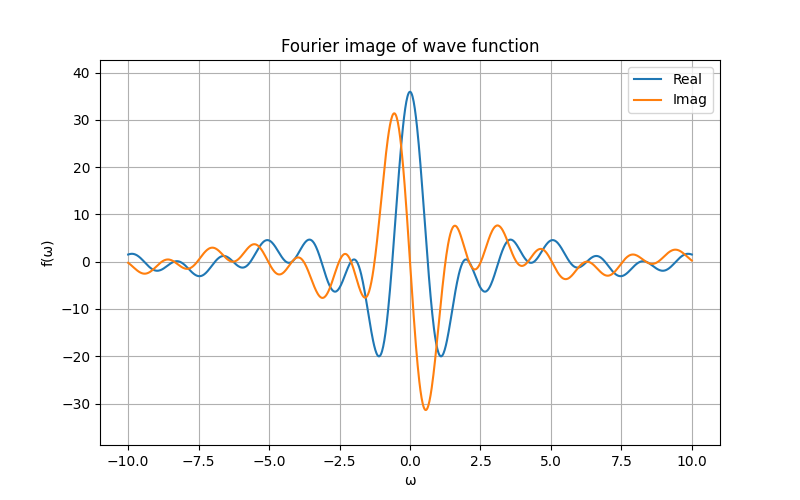
\includegraphics[width=\textwidth]{../results/second/\num/wave_func_image.png}
    \caption{Образ исходной функции $u(t)$.}
    \label{fig:wave_func_image_\num}
\end{figure}

\begin{figure}[ht!]
    \centering
    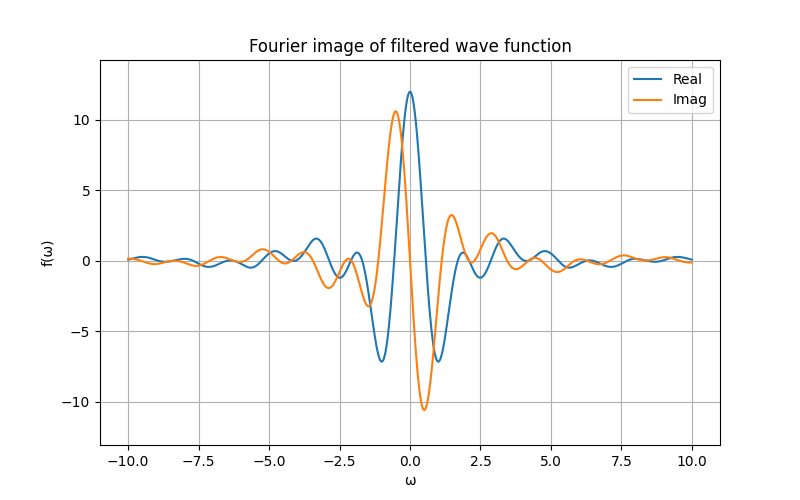
\includegraphics[width=\textwidth]{../results/second/\num/noised_wave_func_filtered_image.png}
    \caption{Образ фильтрованной функции $u'(t)$.}
    \label{fig:noised_wave_func_filtered_image_\num}
\end{figure}

\begin{figure}[ht!]
    \centering
    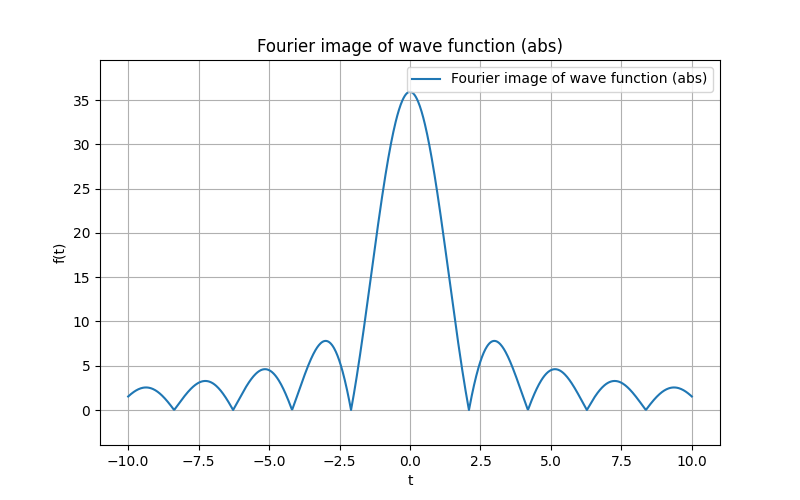
\includegraphics[width=\textwidth]{../results/second/\num/wave_func_image_abs.png}
    \caption{Модуль образа исходной функции $u(t)$.}
    \label{fig:wave_func_image_abs_\num}
\end{figure}

\begin{figure}[ht!]
    \centering
    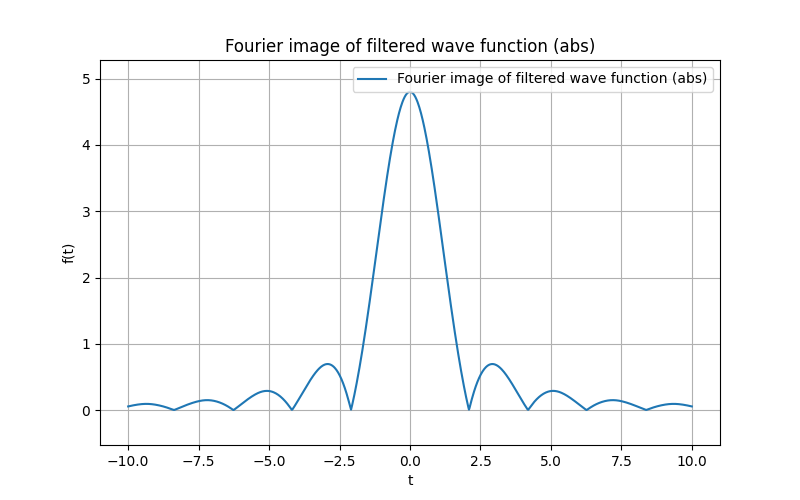
\includegraphics[width=\textwidth]{../results/second/\num/noised_wave_func_filtered_image_abs.png}
    \caption{Модуль образа фильтрованной функции $u'(t)$.}
    \label{fig:noised_wave_func_filtered_image_abs_\num}
\end{figure}

\begin{figure}[ht!]
    \centering
    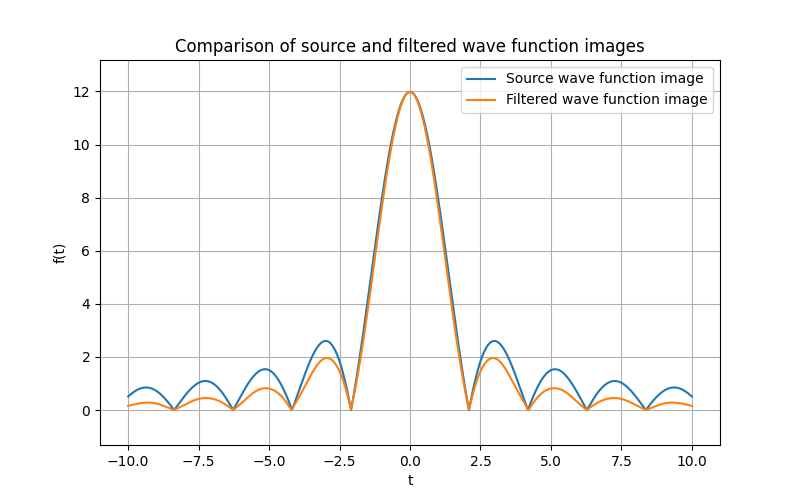
\includegraphics[width=\textwidth]{../results/second/\num/wave_func_image_cmp.png}
    \caption{Сравнение модулей образов исходной и фильтрованной функций.}
    \label{fig:wave_func_image_cmp_\num}
\end{figure}

На графиках модуля исходного и фильтрованного сигнала видно, что фильтр убирает высокочастотные компоненты, что и приводит к сглаживанию функции.

\FloatBarrier
\def\num{2}
\def\T{0.3}
Рассмотрим линейный фильтр первого порядка при $T = \T$ (см. рисунок \ref{fig:noised_wave_func_filtered_\num}).

\begin{figure}[ht!]
    \centering
    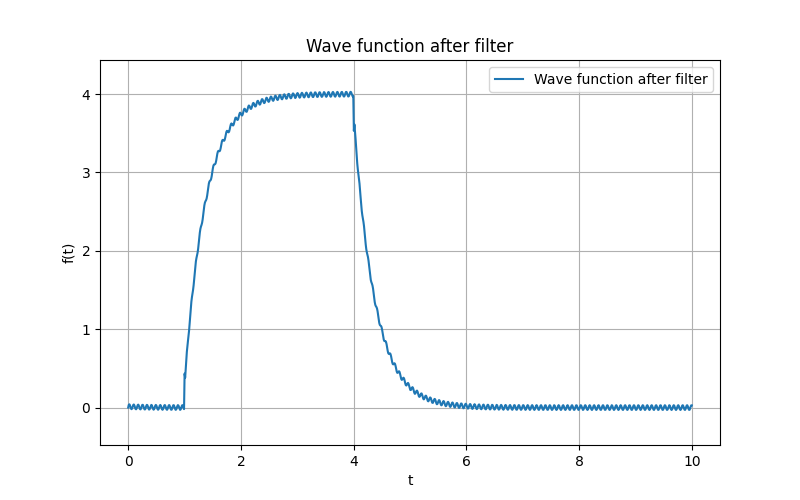
\includegraphics[width=\textwidth]{../results/second/\num/noised_wave_func_filtered.png}
    \caption{Функция $u'(t)$ после применения фильтра}
    \label{fig:noised_wave_func_filtered_\num}
\end{figure}
В данном случае фронт и спад стали более резкими, функция стала больше похожа на исходную. 
АЧХ данного фильтра представлена на рисунке \ref{fig:filter_frequency_response_\num}.

\begin{figure}[ht!]
    \centering
    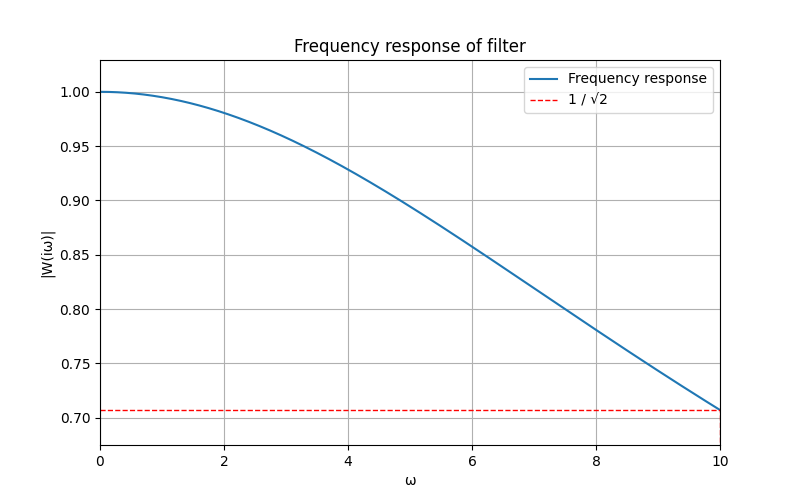
\includegraphics[width=\textwidth]{../results/second/\num/filter_frequency_response.png}
    \caption{АЧХ фильтра первого порядка при $T = \T$}
    \label{fig:filter_frequency_response_\num}
\end{figure}
В данном случае будут подавляться частоты большие $\frac{1}{\T} = \fpeval{round(1/ \T, 3)}$, что значит, что функция лучше повторяет исходную,
по сравнению с прошлой. 

Сравнительный график исходной функции и функции после фильтрации представлен на рисунке \ref{fig:wave_func_cmp_\num}.

Образ исходной функции и функции после фильтрации приведены на рисунках \ref{fig:wave_func_image_\num}~и~\ref{fig:noised_wave_func_filtered_image_\num}.
Графики модулей соответствующих функций приведены на рисунках~\ref{fig:wave_func_image_abs_\num}~и~\ref{fig:noised_wave_func_filtered_image_abs_\num}, их 
сравнительный график -- на рисунке~\ref{fig:wave_func_image_cmp_\num}.

\begin{figure}[ht!]
    \centering
    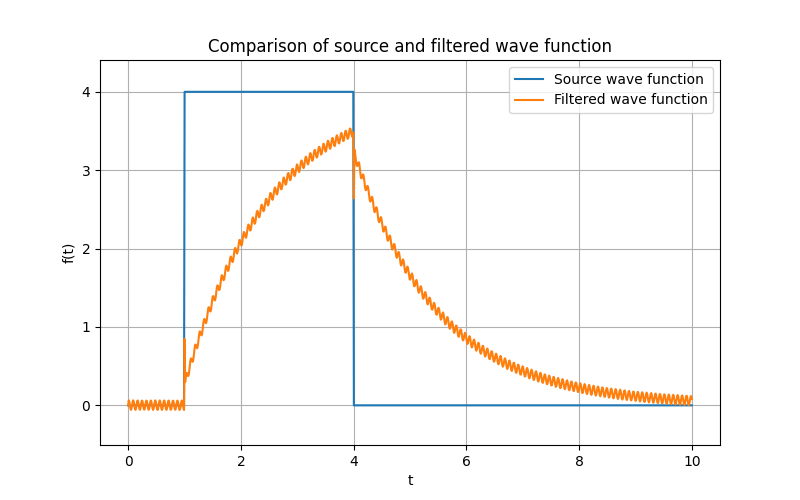
\includegraphics[width=\textwidth]{../results/second/\num/wave_func_cmp.png}
    \caption{Сравнение функции $g(t)$ и $u'(t)$}
    \label{fig:wave_func_cmp_\num}
\end{figure}

\begin{figure}[ht!]
    \centering
    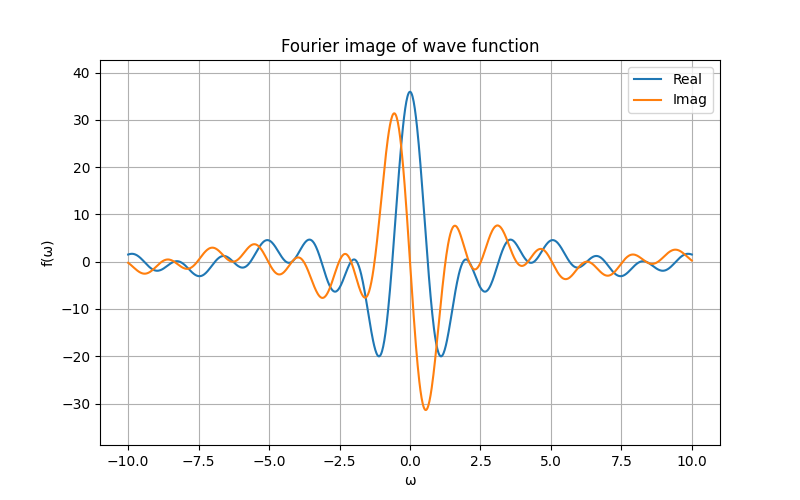
\includegraphics[width=\textwidth]{../results/second/\num/wave_func_image.png}
    \caption{Образ исходной функции $u(t)$.}
    \label{fig:wave_func_image_\num}
\end{figure}

\begin{figure}[ht!]
    \centering
    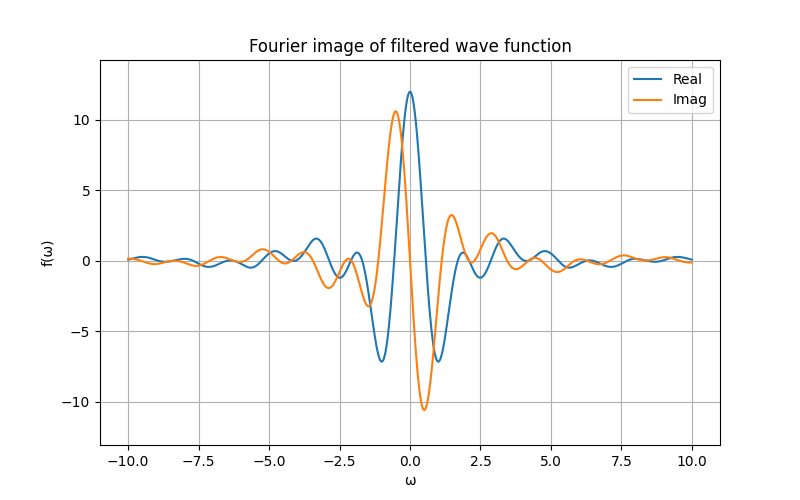
\includegraphics[width=\textwidth]{../results/second/\num/noised_wave_func_filtered_image.png}
    \caption{Образ фильтрованной функции $u'(t)$.}
    \label{fig:noised_wave_func_filtered_image_\num}
\end{figure}

\begin{figure}[ht!]
    \centering
    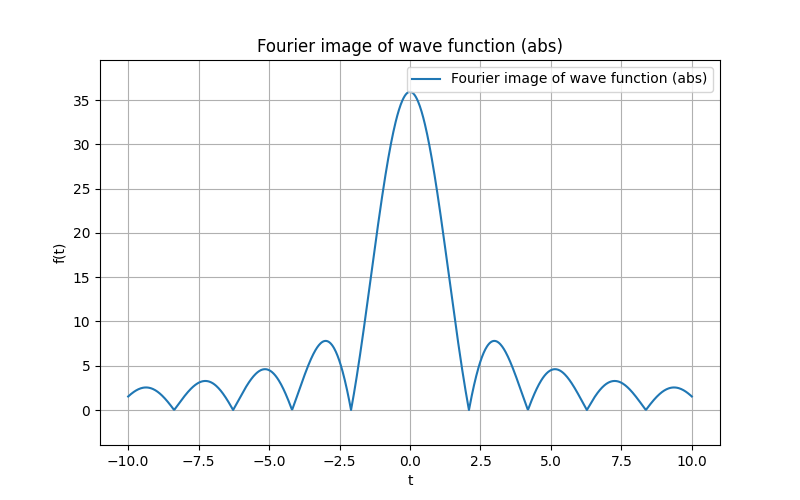
\includegraphics[width=\textwidth]{../results/second/\num/wave_func_image_abs.png}
    \caption{Модуль образа исходной функции $u(t)$.}
    \label{fig:wave_func_image_abs_\num}
\end{figure}

\begin{figure}[ht!]
    \centering
    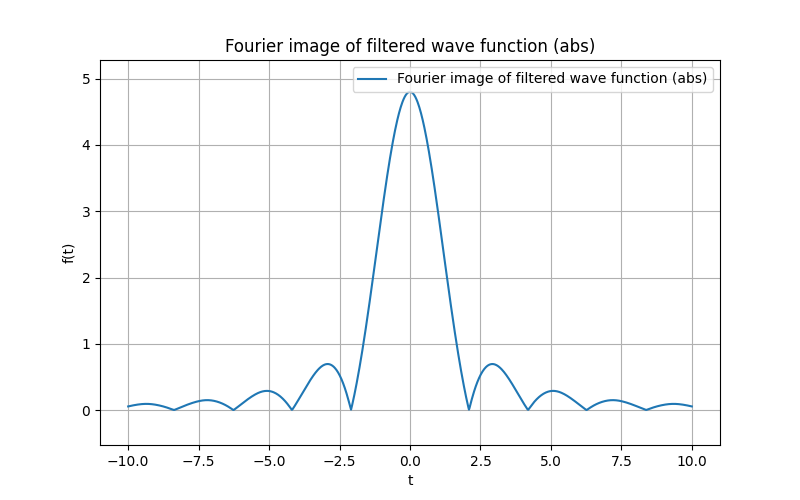
\includegraphics[width=\textwidth]{../results/second/\num/noised_wave_func_filtered_image_abs.png}
    \caption{Модуль образа фильтрованной функции $u'(t)$.}
    \label{fig:noised_wave_func_filtered_image_abs_\num}
\end{figure}

\begin{figure}[ht!]
    \centering
    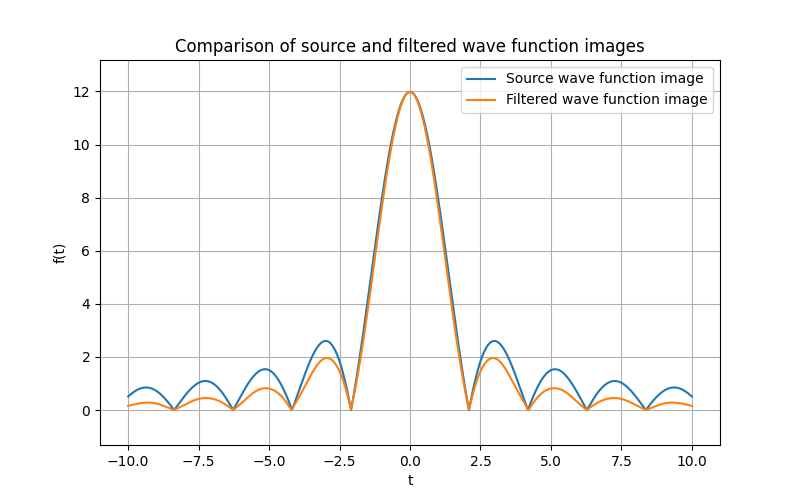
\includegraphics[width=\textwidth]{../results/second/\num/wave_func_image_cmp.png}
    \caption{Сравнение модулей образов исходной и фильтрованной функций.}
    \label{fig:wave_func_image_cmp_\num}
\end{figure}


\FloatBarrier
\def\num{3}
\def\T{0.1}
Также посмотрим на фильтр с параметром $T = \T$ (см. рисунок \ref{fig:noised_wave_func_filtered_\num}).
\begin{figure}[ht!]
    \centering
    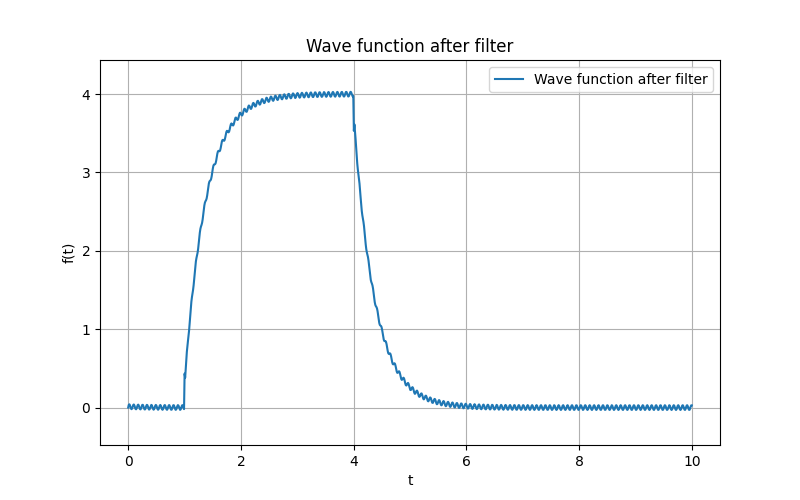
\includegraphics[width=\textwidth]{../results/second/\num/noised_wave_func_filtered.png}
    \caption{Функция $u'(t)$ после применения фильтра}
    \label{fig:noised_wave_func_filtered_\num}
\end{figure}
Теперь функция стала еще более похожей на исходную квадратную волну, но в фильтрованной функции 
стали проявляться шумы из исходной функции. 
АЧХ данного фильтра представлена на рисунке \ref{fig:filter_frequency_response_\num}.

\begin{figure}[ht!]
    \centering
    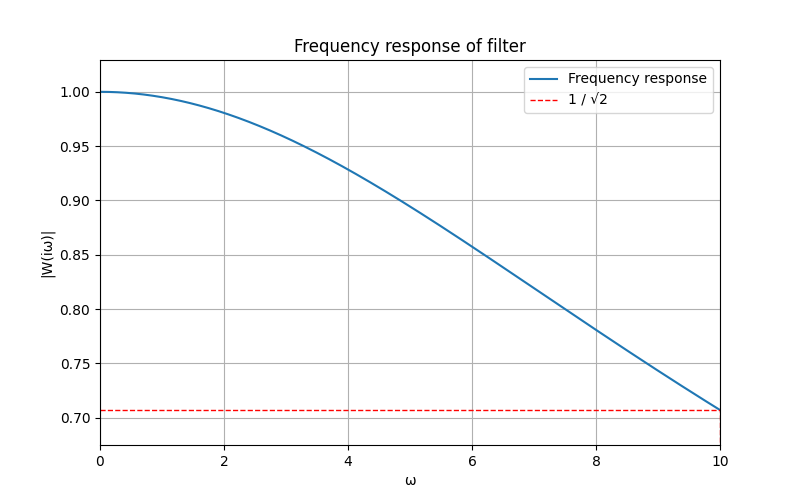
\includegraphics[width=\textwidth]{../results/second/\num/filter_frequency_response.png}
    \caption{АЧХ фильтра первого порядка при $T = \T$}
    \label{fig:filter_frequency_response_\num}
\end{figure}

Сравнительный график исходной функции и функции после фильтрации представлен на рисунке \ref{fig:wave_func_cmp_\num}.

\begin{figure}[ht!]
    \centering
    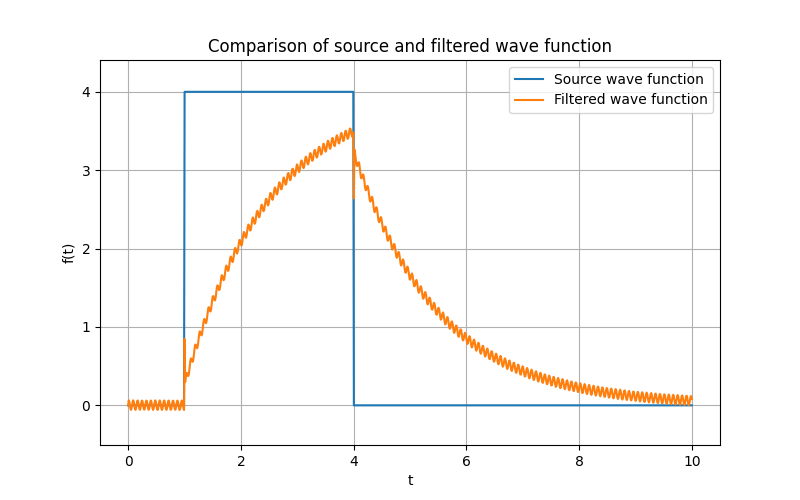
\includegraphics[width=\textwidth]{../results/second/\num/wave_func_cmp.png}
    \caption{Сравнение функции $g(t)$ и $u'(t)$}
    \label{fig:wave_func_cmp_\num}
\end{figure}

Можем сделать вывод, что при увеличении постоянной времени $T$ фильтра, функция становится более гладкой,
при этом меньше похожей на исходную. 

Образ исходной функции и функции после фильтрации приведены на рисунках \ref{fig:wave_func_image_\num}~и~\ref{fig:noised_wave_func_filtered_image_\num}.
Графики модулей соответствующих функций приведены на рисунках~\ref{fig:wave_func_image_abs_\num}~и~\ref{fig:noised_wave_func_filtered_image_abs_\num}, их 
сравнительный график -- на рисунке~\ref{fig:wave_func_image_cmp_\num}.

\begin{figure}[ht!]
    \centering
    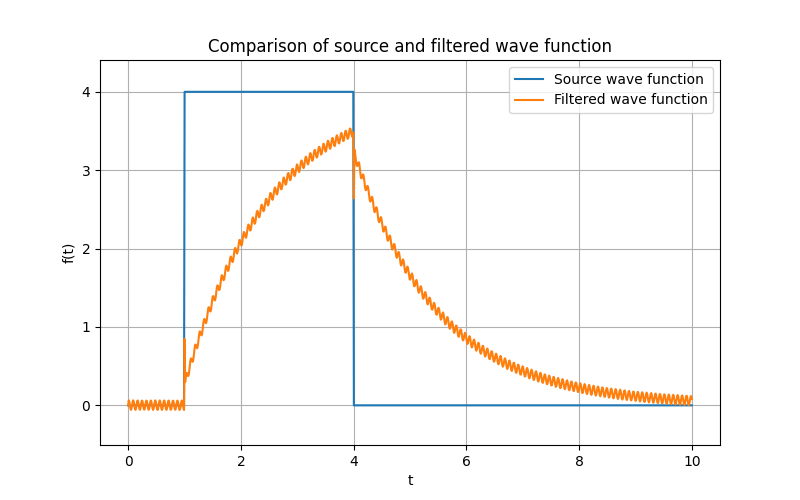
\includegraphics[width=\textwidth]{../results/second/\num/wave_func_cmp.png}
    \caption{Сравнение функции $g(t)$ и $u'(t)$}
    \label{fig:wave_func_cmp_\num}
\end{figure}

\begin{figure}[ht!]
    \centering
    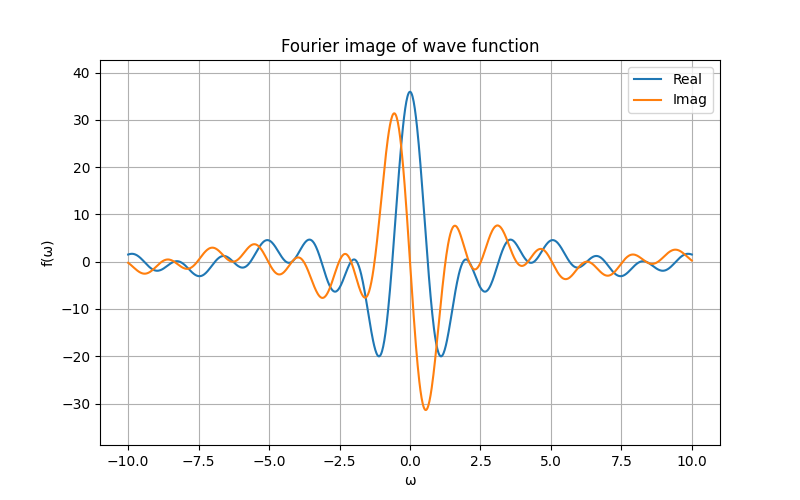
\includegraphics[width=\textwidth]{../results/second/\num/wave_func_image.png}
    \caption{Образ исходной функции $u(t)$.}
    \label{fig:wave_func_image_\num}
\end{figure}

\begin{figure}[ht!]
    \centering
    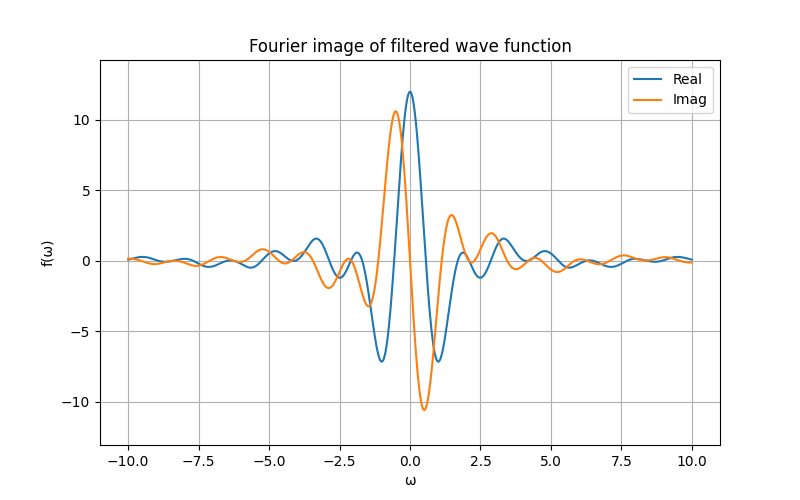
\includegraphics[width=\textwidth]{../results/second/\num/noised_wave_func_filtered_image.png}
    \caption{Образ фильтрованной функции $u'(t)$.}
    \label{fig:noised_wave_func_filtered_image_\num}
\end{figure}

\begin{figure}[ht!]
    \centering
    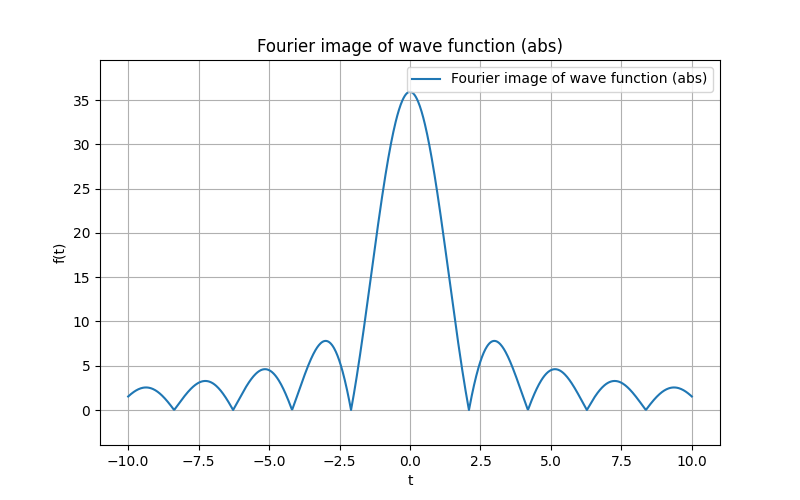
\includegraphics[width=\textwidth]{../results/second/\num/wave_func_image_abs.png}
    \caption{Модуль образа исходной функции $u(t)$.}
    \label{fig:wave_func_image_abs_\num}
\end{figure}

\begin{figure}[ht!]
    \centering
    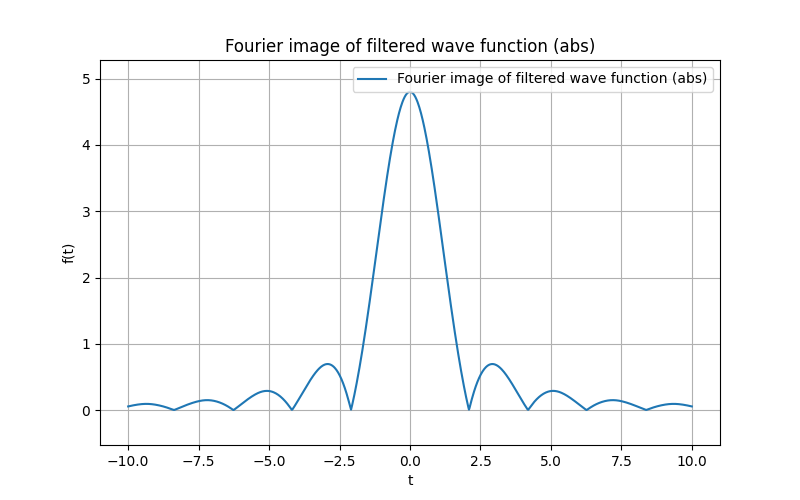
\includegraphics[width=\textwidth]{../results/second/\num/noised_wave_func_filtered_image_abs.png}
    \caption{Модуль образа фильтрованной функции $u'(t)$.}
    \label{fig:noised_wave_func_filtered_image_abs_\num}
\end{figure}

\begin{figure}[ht!]
    \centering
    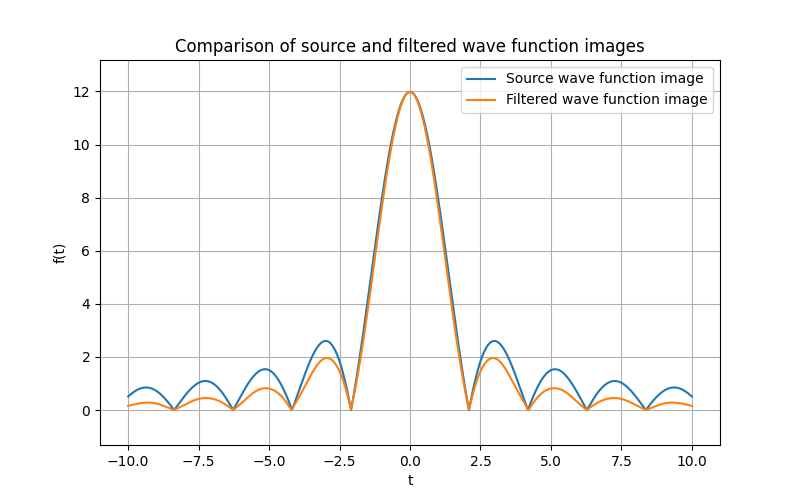
\includegraphics[width=\textwidth]{../results/second/\num/wave_func_image_cmp.png}
    \caption{Сравнение модулей образов исходной и фильтрованной функций.}
    \label{fig:wave_func_image_cmp_\num}
\end{figure}


\FloatBarrier
\subsubsection{Зависимость эффективности фильтрации от параметра a}
\def\T{0.3}
Для исследования данной зависимости рассмотрим функцию $g(t)$ при различных значениях параметра $a$ 
при фильтрации линейным фильтром первого порядка с $T = \T$. 

\def\num{4}
\def\a{10}
Рассмотрим функцию $g(t)$ при параметрах $a=\a$, $t_1 = \from$, $t_2 = \to$ ~(см. рисунок~\ref{fig:wave_func_\num}) 
и ее \textit{зашумленную} версию $u(t)$ с параметрами $b = \b$, $c = \c$, $d = \d$ ~(см. рисунок~\ref{fig:noised_wave_func_\num}).
на промежутке $[0,\L]$. 

\begin{figure}[ht!]
    \centering
    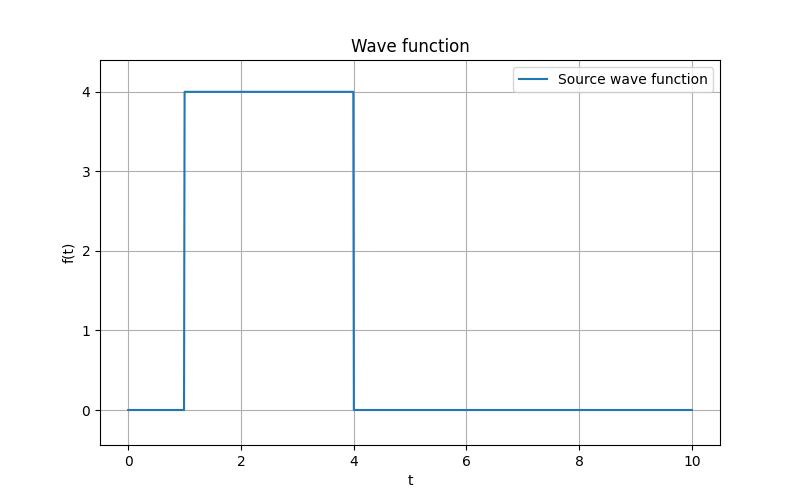
\includegraphics[width=\textwidth]{../results/second/\num/wave_func.png}
    \caption{Функция $g(t)$ с параметрами $a = \a$, $t_1 = \from$, $t_2 = \to$}
    \label{fig:wave_func_\num}
\end{figure}

\begin{figure}[ht!]
    \centering
    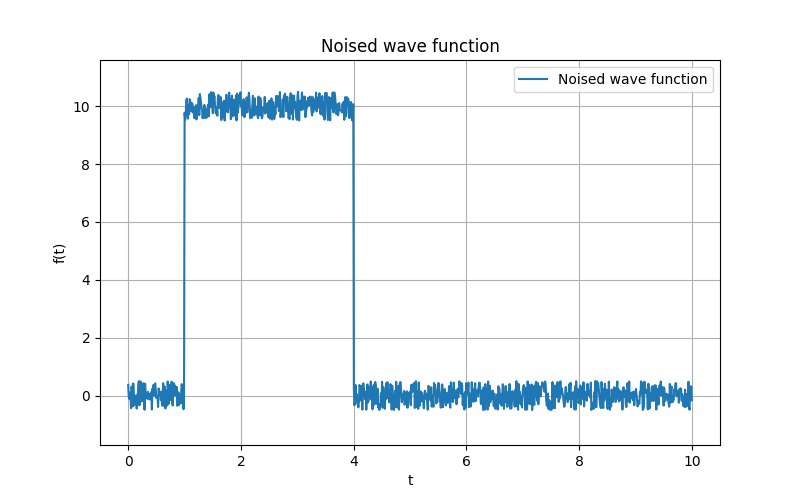
\includegraphics[width=\textwidth]{../results/second/\num/noised_wave_func.png}
    \caption{Функция $u(t)$ с параметрами $b = \b$, $c = \c$, $d = \d$}
    \label{fig:noised_wave_func_\num}
\end{figure}

Результат фильтрации с помощью линейного фильтра первого порядка с $T = \T$ (см. рисунок \ref{fig:noised_wave_func_filtered_\num}).
Сравнительные графики исходной функции и функции после фильтрации представлены на рисунке \ref{fig:wave_func_cmp_\num}.

\begin{figure}[ht!]
    \centering
    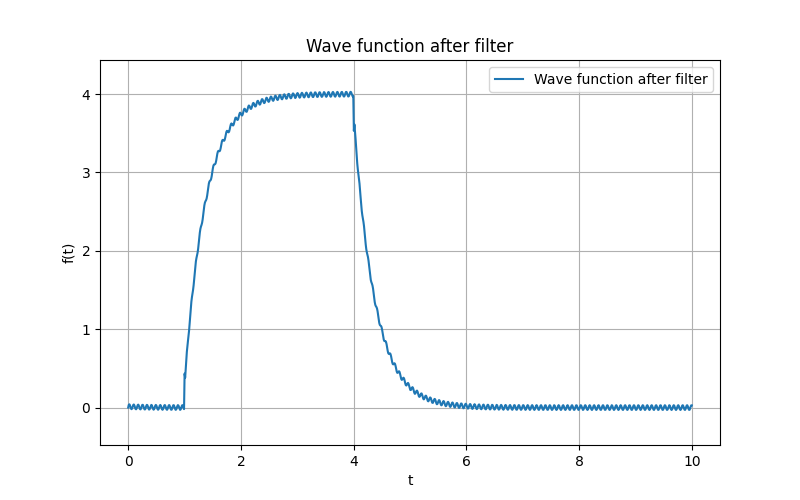
\includegraphics[width=\textwidth]{../results/second/\num/noised_wave_func_filtered.png}
    \caption{Функция $u'(t)$ после применения фильтра}
    \label{fig:noised_wave_func_filtered_\num}
\end{figure}

\begin{figure}[ht!]
    \centering
    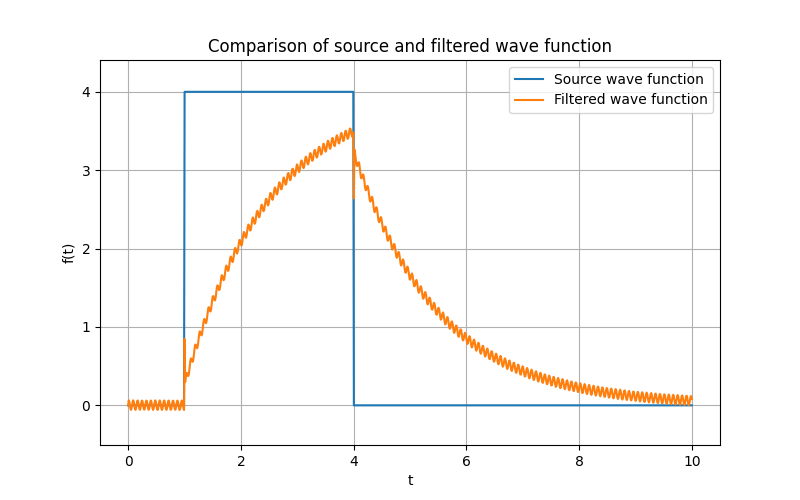
\includegraphics[width=\textwidth]{../results/second/\num/wave_func_cmp.png}
    \caption{Сравнение функции $g(t)$ и $u'(t)$}
    \label{fig:wave_func_cmp_\num}
\end{figure}

Результат практически не отличается от предыдущего случая. Функция стала более гладкой, но при этом
менее похожей на исходную. Фронт и спад так же завалены. 

\def\num{5}
\def\a{30}
Рассмотрим функцию $g(t)$ при параметрах $a=\a$, $t_1 = \from$, $t_2 = \to$ ~(см. рисунок~\ref{fig:wave_func_\num}) 
и ее \textit{зашумленную} версию $u(t)$ с параметрами $b = \b$, $c = \c$, $d = \d$ ~(см. рисунок~\ref{fig:noised_wave_func_\num}).
на промежутке $[0,\L]$. 

\begin{figure}[ht!]
    \centering
    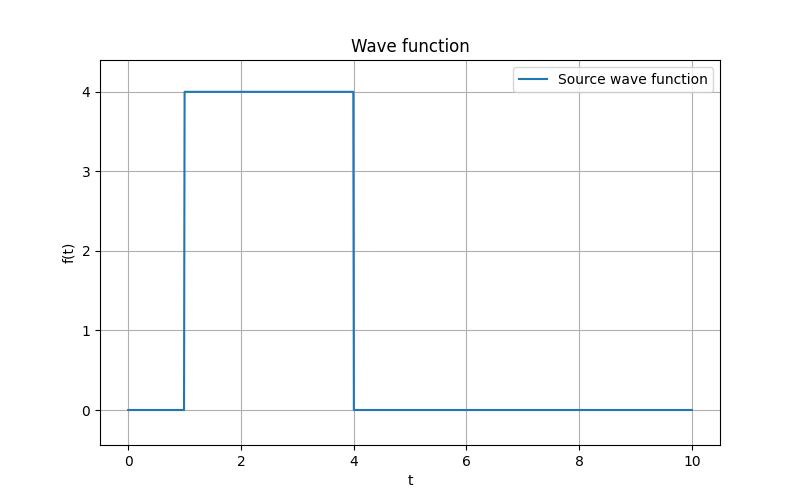
\includegraphics[width=\textwidth]{../results/second/\num/wave_func.png}
    \caption{Функция $g(t)$ с параметрами $a = \a$, $t_1 = \from$, $t_2 = \to$}
    \label{fig:wave_func_\num}
\end{figure}

\begin{figure}[ht!]
    \centering
    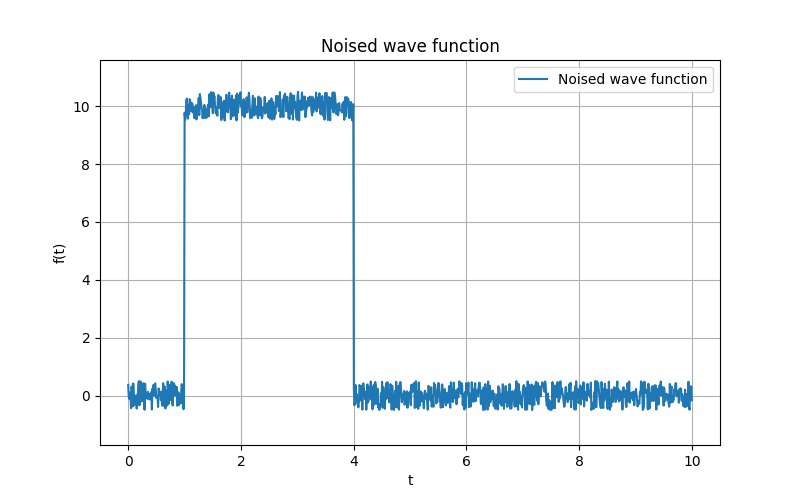
\includegraphics[width=\textwidth]{../results/second/\num/noised_wave_func.png}
    \caption{Функция $u(t)$ с параметрами $b = \b$, $c = \c$, $d = \d$}
    \label{fig:noised_wave_func_\num}
\end{figure}

Результат фильтрации с помощью линейного фильтра первого порядка с $T = \T$ (см. рисунок \ref{fig:noised_wave_func_filtered_\num}).

\begin{figure}[ht!]
    \centering
    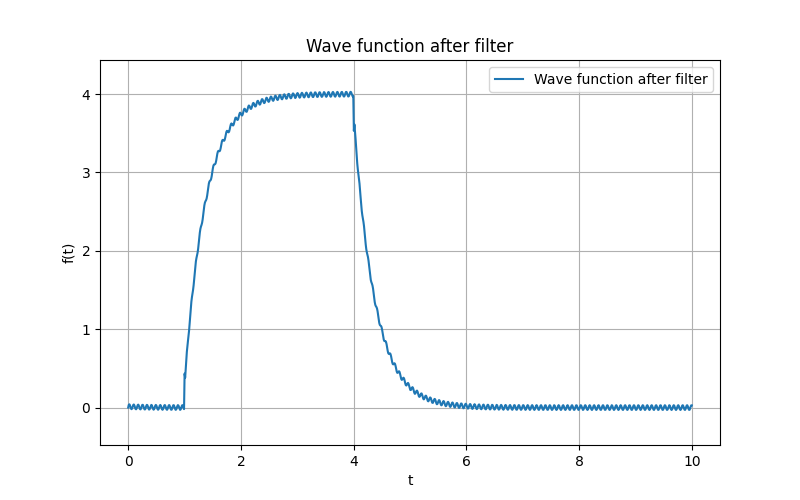
\includegraphics[width=\textwidth]{../results/second/\num/noised_wave_func_filtered.png}
    \caption{Функция $u'(t)$ после применения фильтра}
    \label{fig:noised_wave_func_filtered_\num}
\end{figure}

\begin{figure}[ht!]
    \centering
    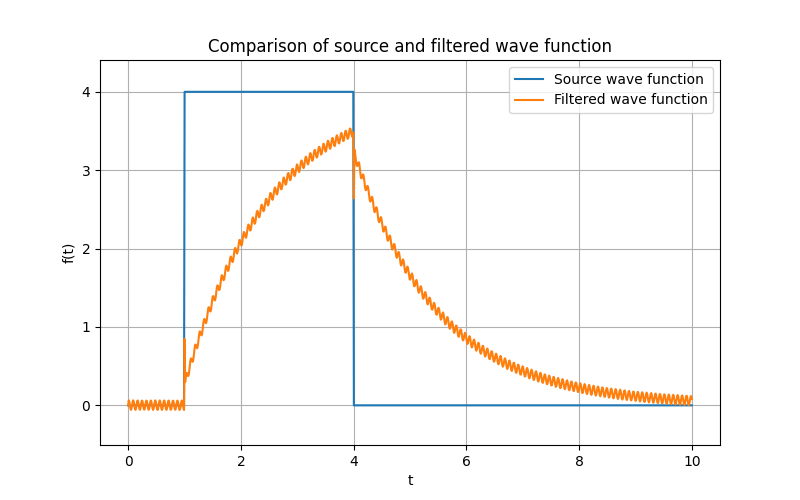
\includegraphics[width=\textwidth]{../results/second/\num/wave_func_cmp.png}
    \caption{Сравнение функции $g(t)$ и $u'(t)$}
    \label{fig:wave_func_cmp_\num}
\end{figure}

Ровно как и в прошлый раз -- никаких изменений. Фронт функции выглядит идентично с поправкой на масштаб.
Сравнительные графики исходной функции и функции после фильтрации представлены на рисунке \ref{fig:wave_func_cmp_\num}.

Можно сделать вывод, что параметр $a$ не влияет на эффективность фильтрации линейным фильтром первого порядка. 
Связано это с тем, что, фильтр первого порядка лишь \textit{масштабирует} функцию согласно его АЧХ. 
